\documentclass[]{ximera}
%handout:  for handout version with no solutions or instructor notes
%handout,instructornotes:  for instructor version with just problems and notes, no solutions
%noinstructornotes:  shows only problem and solutions

%% handout
%% space
%% newpage
%% numbers
%% nooutcomes

%I added the commands here so that I would't have to keep looking them up
%\newcommand{\RR}{\mathbb R}
%\renewcommand{\d}{\,d}
%\newcommand{\dd}[2][]{\frac{d #1}{d #2}}
%\renewcommand{\l}{\ell}
%\newcommand{\ddx}{\frac{d}{dx}}
%\everymath{\displaystyle}
%\newcommand{\dfn}{\textbf}
%\newcommand{\eval}[1]{\bigg[ #1 \bigg]}

%\begin{image}
%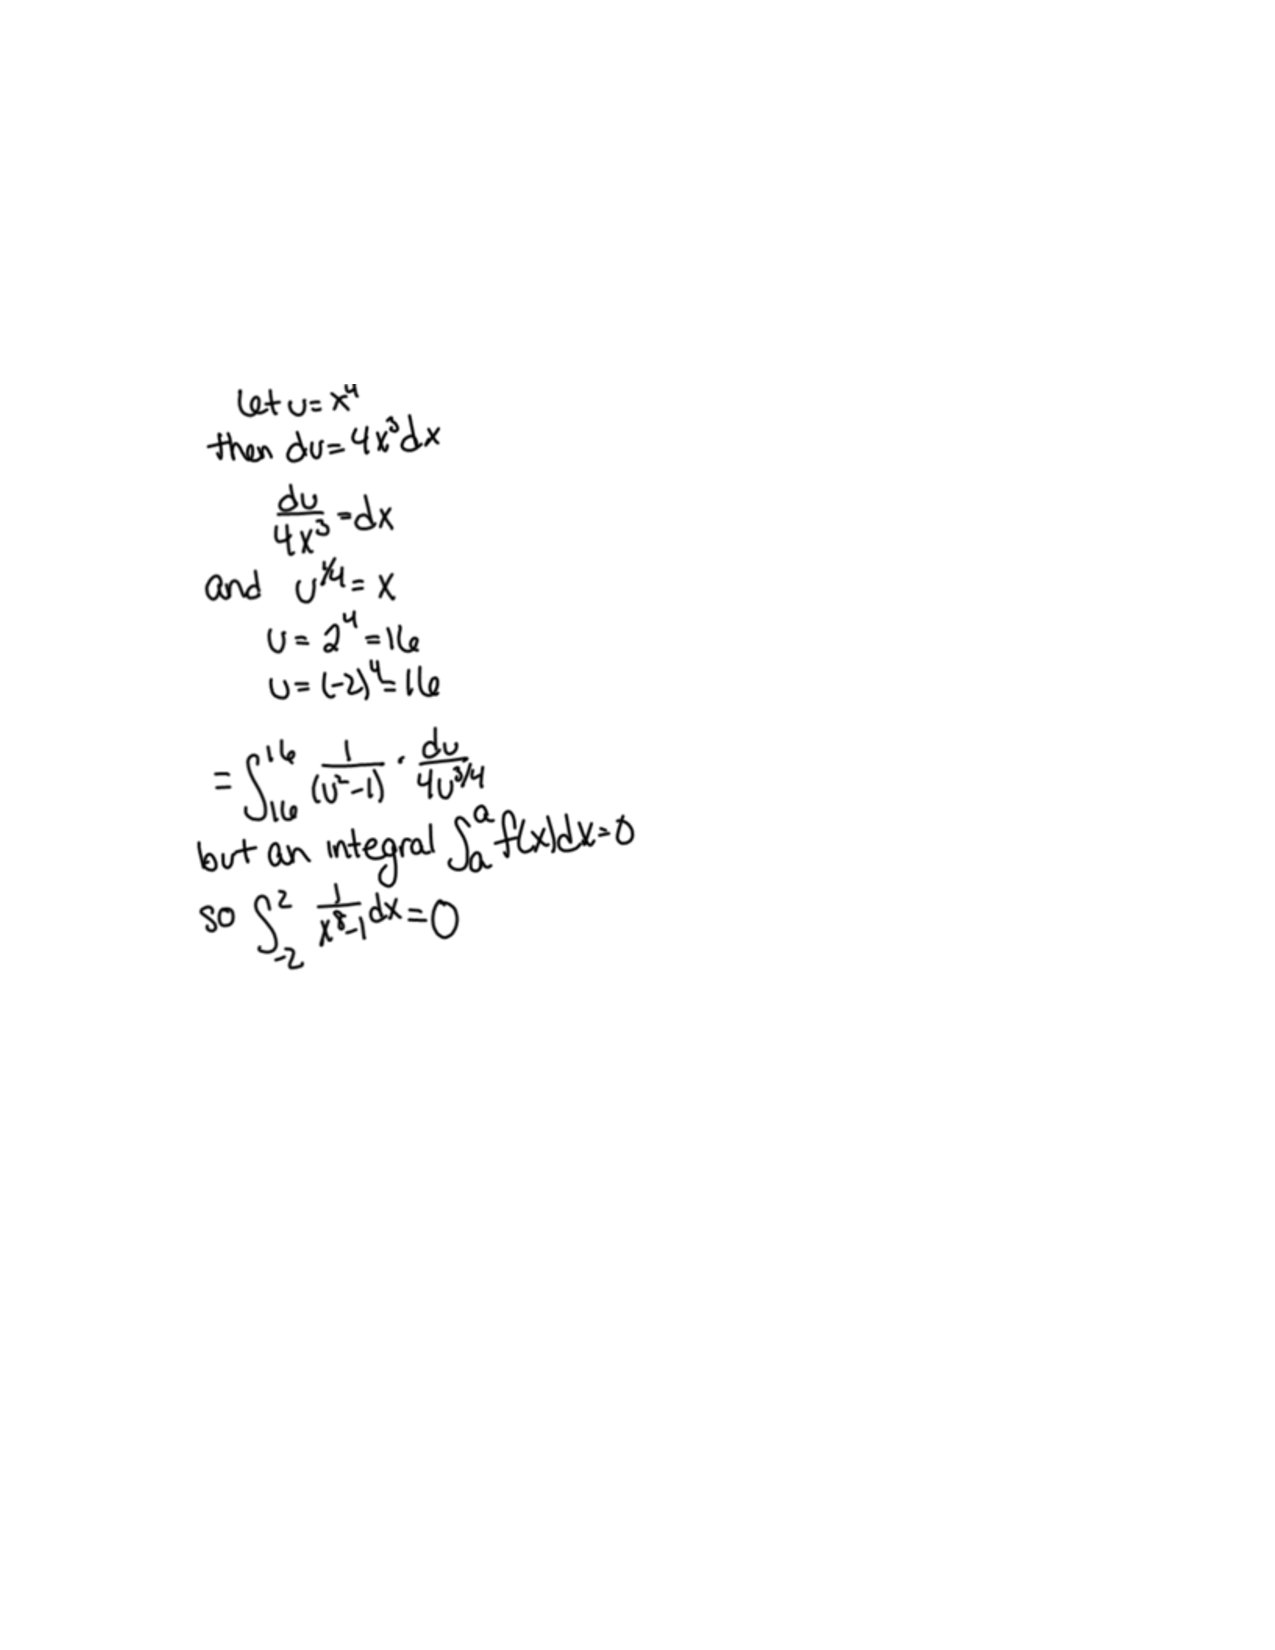
\includegraphics[trim= 170 420 250 180]{Figure1.pdf}
%\end{image}

%add a ``.'' below when used in a specific directory.
\newcommand{\RR}{\mathbb R}
\renewcommand{\d}{\,d}
\newcommand{\dd}[2][]{\frac{d #1}{d #2}}
\renewcommand{\l}{\ell}
\newcommand{\ddx}{\frac{d}{dx}}
\newcommand{\dfn}{\textbf}
\newcommand{\eval}[1]{\bigg[ #1 \bigg]}

\usepackage{multicol}

\renewenvironment{freeResponse}{
\ifhandout\setbox0\vbox\bgroup\else
\begin{trivlist}\item[\hskip \labelsep\bfseries Solution:\hspace{2ex}]
\fi}
{\ifhandout\egroup\else
\end{trivlist}
\fi} %% we can turn off input when making a master document

\title{Taylor series}  

\begin{document}
\begin{abstract}		\end{abstract}
\maketitle



\section{Warm up:}
Find the Taylor series for:  
	\begin{enumerate}
	\item  $27x^2 - 3x + 17$ about $a=1$.  
	\item  $\sin(2x)$ about $a = \frac{\pi}{8}$.  
	\end{enumerate}
	
	\begin{freeResponse}
	\begin{enumerate}
	\item
	\item
	\end{enumerate}
	\end{freeResponse}
	
\begin{instructorNotes}
Here, they need to compute the Taylor series by computing derivatives and recognizing patterns.  

Part (a) is an opportunity to show the students that a polynomial is already a Maclaurin series.  
Use derivatives to figure out the Taylor series about $a=1$, and then show them that the answer simplifies back to the original problem.  

Part (b) is a continuation from the previous recitation where they already found the approximating polynomial.  
The students may have a problem finding the pattern in the derivatives.
\end{instructorNotes}







\section{Group work:}



%problem 1
\begin{problem}
Find a power series (and interval of convergence) for each of the following functions
	\begin{multicols}{2}
	\begin{enumerate}
	\item  $f(x) = x^3 \sin(x^5)$
	\item  $f(x) = \frac{1}{(1+x)^4}$
	\item  $f(x) = \frac{1}{(3-5x^2)^4}$
	\item  $f(x) = \sin^{-1}(x^5)$
	\end{enumerate}
	\end{multicols}
	
	\begin{freeResponse}
	\begin{enumerate}
	\item
	
	\item
	
	\item
	
	\item
	
	\end{enumerate}
	\end{freeResponse}
	
\end{problem}

\begin{instructorNotes}
Students should use the known Maclaurin series in various ways.  
You might want to give the hint in part (d) that $\ddx \sin^{-1}(x) = \frac{1}{\sqrt{1-x^2}}$.  
\end{instructorNotes}







%problem 2
\begin{problem}
Find a function (closed expression) for the following series and the interval on which the function and the series are equal.
	\[
	x + x^4 + \frac{1}{2} x^7 + \frac{1}{6} x^{10} + \frac{1}{24} x^{13} + \hdots
	\]
	\begin{freeResponse}
	
	\end{freeResponse}
		
\end{problem}

\begin{instructorNotes}
The students need to rewrite $f(x)$ in summation notation (factoring out an $x$) and seeing the series for $xe^{x^3}$.  
\end{instructorNotes}







%problem 3
\begin{problem}
Compute the sum of the following series ({\it Hint:  You should use Taylor series.})
	\begin{enumerate}
	\item  $1 - \ln 2 + \frac{(\ln 2)^2}{2!} - \frac{(\ln 2)^3}{3!} + \hdots$
	\item  $3 + \frac{9}{2!} + \frac{27}{3!} + \frac{81}{4!} + \hdots$
	\end{enumerate}
	
	\begin{freeResponse}
	\begin{enumerate}
	\item  
	\item  
	\end{enumerate}
	\end{freeResponse}

\end{problem}

\begin{instructorNotes}
The goal here is for students to realize that Taylor series gives them a tool for finding the exact sum of a series.
\end{instructorNotes}
















	
	
	
	
	
	
	
	
	

	










								
				
				
	














\end{document} 


















